\section{Grafteori}

Grafteori handler om at beskrive  modeller matematisk. Grafteori er væslig når man skal optimere et netværk, det kunne f.eks. være en graf som representere et vejnetværk, hvor man her vil kunne bruge grafteori til bla rutefinding.  

En graf beskriver et par af mægnder, man kunne tag udgangspunkt i grafen G = (V,E) hvor V og E er mægnder. I eksempet her er V en ikke-tom mængde af knuder, og E er mængden af kanter som forbinder knuderne i mægnden V. 

\vspace{5mm}

Vi tager udgangpunkt i grafen på figur \ref{fig:weighted-directed-graph}.

\begin{figure}[H]
\begin{adjustbox}{width=0.5\textwidth,center=\textwidth}
\centering
\includegraphics[width=0.5\textwidth]{Pictures/Teoriafsnit/Figurfiler/weighted_directed_graph.PNG}
\end{adjustbox}
\caption{Orienteret vægtet graf}
\label{fig:weighted-directed-graph}
\end{figure}

\vspace{5mm}

Man kan forstille sig dette er et vejnetværk, hvor knuderne repræsentere sving, og linjerne er veje som forbinder svingene, samt beskriver tallet mellem 2 knuder længden af vejen. Herved kan grafen godt forstille et simpel vejnetværk.

\vspace{5mm}

Vi kan ud fra grafen se at knuderne \verb!"A, B, C, D, E, F \in V"!. 

\vspace{5mm}

Samt at kanterne
\begin{equation}\label{grafteori}
\begin{split}
\{A,B\} \rightarrow 4, \{A,F\} \rightarrow 5, \{B,D\} \rightarrow 7, \{C,A\} \rightarrow 3, \{C,B\} \rightarrow 4, \{D,C\} \rightarrow 2, \\ 
\{D,E\} \rightarrow 3, \{E,D\} \rightarrow 3, \{E,F\} \rightarrow 2, \{F,C\} \rightarrow 1, \{F,E\} \rightarrow 1 \in E.
\end{split}
\end{equation}

\vspace{5mm}

Grafen her kan derfor skrives rent matematisk:

\vspace{5mm}

\verb!G = (V,E), V = {A,B,C,D,E,F},! 

\vspace{5mm}

\begin{equation}\label{grafteori}
\begin{split}
E = \{ \{A,B\} \rightarrow 4, \{A,F\} \rightarrow 5, \{B,D\} \rightarrow 7, \{C,A\} \rightarrow 3, \{C,B\} \rightarrow 4, \{D,C\} \rightarrow 2, \\
 \{D,E\}  \rightarrow 3, \{E,D\} \rightarrow 3, \{E,F\} \rightarrow 2, \{F,C\} \rightarrow 1, \{F,E\} \rightarrow 1 \in  E\}
\end{split}
\end{equation}

\vspace{5mm}

En anden måde at repræsentere grafen på er ved hjælp af en nabo-matrix VxE, hvor v1, v2...vn, er knuderne, og e1, e2...en, er kanterne. Se figur \ref{fig:adjacency-matrix-weighted-directed-graph}. 

I matrixen beskrives forbindelser mellem 2 knuder med et tal, og knudere uden forbindelse beskrives med $\infty$. Man vil altså derfor kunne tegne en graf alene ud fra matrixens værdier.

\begin{figure}[H]
\begin{adjustbox}{width=0.5\textwidth,center=\textwidth}
\centering
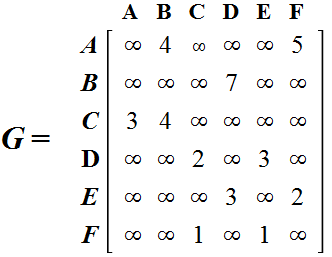
\includegraphics[width=0.5\textwidth]{Pictures/Teoriafsnit/Figurfiler/adjacency_matrix_weighted_directed_graph.PNG}
\end{adjustbox}
\caption{Nabo Matrix af orienteret vægtet graf}
\label{fig:adjacency-matrix-weighted-directed-graph}
\end{figure}

Grafteori er et vigtigt emne, da f.eks. korteste rute algoritmer som Dijkstra's har brug for at vide hvordan knuderne er forbundet, samt graden(hvor mange kanter knuden har) af den enktle knude, for at kun udregne den korteste rute. Derudover vil en grafmetode som en nabo-matix være en god måde at beskrive et vejnætværk på programerings niveau, da man kan have alle sine værdier i en variable. \cite{Grafteori1} \cite{Grafteori2}


